\newpage

\section{Problem Definition}
\label{sec:problem-definition}

\newcommand{\grammartag}[1]{\qquad\qquad\emph{(#1)}}
\begin{figure}[t]
    \begin{align*}
    \mathbf{Expression}\quad e ::= &&& \\
       | & \quad 0 \mid 1 \mid 2 \mid \ldots                                && \grammartag{Numeric constants} \\
       | & \quad \nondet                                 && \grammartag{Nondeterministic value: 0 or 1}\\
       | & \quad x := e                            && \grammartag{Write to local packet field} \\
       | & \quad x                                 && \grammartag{Read from local packet field} \\
       | & \quad X := e                            && \grammartag{Write to global switch variable} \\
       | & \quad X                                 && \grammartag{Read from global switch variable} \\
       | & \quad e_1 == e_2                        && \grammartag{Equality test} \\
       | & \quad e_1 ; e_2                         && \grammartag{Sequencing} \\
       | & \quad \ifkw(e_1)\{\ e_2\ \}\elsekw\{\ e_3\ \} && \grammartag{Conditional} \\
       | & \quad \whilekw(e_1)\{\ e_2\ \}              && \grammartag{While loop} \\
       | & \quad \yieldkw                      && \grammartag{Yields to scheduler}\\[1em]
    \mathbf{Program}\quad p ::=
        & \quad \requestkw\ name_1\ \{\ e_1\ \}&&\grammartag{Set of request handlers}\\[-0.5em]
        & \quad \qquad \vdots &&\\
        & \quad \requestkw\ name_n\ \{\ e_n\ \}\ 
    \end{align*}
    \caption{Syntax of expressians and programs}
    \label{fig:syntax}
\end{figure}
    
A Network System $\mathcal{N}$ is a tuple $(G, L, \mathit{Req}, \mathit{Res}, g_0, \delta, \mathit{req}, \mathit{resp})$ where:
\begin{itemize}
\item $G$ is a set of global states representing switch state
\item $L$ is a set of local states representing packet contents
\item $\mathit{Req}$ is a set of request events
\item $\mathit{Res}$ is a set of response events
\item $g_0 \in G$ is the initial global state
\item $\mathit{req} \subseteq \mathit{Req} \times L$ is a request transition relation, which describes which requests turn into which packets
\item $\mathit{resp} \subseteq L \times \mathit{Res}$ is a response transition relation, which describes which packets turn into which responses
\item $\delta \subseteq (G \times L) \times (G \times L)$ is a transition relation for packet processing, which describes an atomic step of packet processing that may change the global state.
\end{itemize}

\begin{figure}[t]
    \centering
    \renewcommand{\arraystretch}{1.6}
    \[
    \begin{array}{c}
    \textbf{States and Transitions:}
    \\
    \quad
    \text{A (global) \emph{network state} is a triple }(g,\mathcal{P},M)\text{ where:}
    \\
    \quad
    g \in G \text{ is the current global switch state,}
    \\
    \quad
    \mathcal{P} \in \text{Multiset}(L \times \mathit{Req}) \text{ is a multiset of in-flight packets,}
    \\
    \quad
    M \in \text{Multiset}(\mathit{Req} \times \mathit{Res}) \text{ is a multiset of request--response pairs already completed.}
    \end{array}
    \]

    \[
    \begin{array}{c}
    \textbf{Initial state:}
    \\
    \quad (g_0,\,\varnothing,\,\varnothing)
    \end{array}
    \]

    \[
    \begin{array}{c}
    \textbf{Transition rules:}
    \\[1em]
    \text{(New Request)}\quad\infer{
    (r,\ell)\,\in\,\mathit{req}
    }
    {(g,\;\mathcal{P},\;M) \;\longrightarrow\; (g,\;\mathcal{P} \uplus \{(\ell,r)\},\;M)}
    \\[2em]
    \text{(Packet Step)}\quad\infer{
    ((g,\ell),\,(g',\ell')) \,\in\, \delta
    }
    {(g,\;\mathcal{P} \uplus \{(\ell,r)\},\;M) \;\longrightarrow\; (g',\;\mathcal{P} \uplus \{(\ell',r)\},\;M)}
    \\[2em]
    \text{(Response)}\quad\infer{
    (\ell,s)\,\in\,\mathit{resp}
    }
    {(g,\;\mathcal{P} \uplus \{(\ell,r)\},\;M) \;\longrightarrow\; (g,\;\mathcal{P},\;M \uplus \{(r,s)\})}
    \end{array}
    \]

    \[
    \begin{array}{c}
    \textbf{Complete runs:}
    \\
    \quad (g_0,\,\varnothing,\,\varnothing) \;\longrightarrow\; (g_1,\,\mathcal{P}_1,\,M_1) \;\longrightarrow\; \cdots \;\longrightarrow\; (g_n,\,\mathcal{P}_{n-1},\,M_{n-1}) \;\longrightarrow\; (g_n,\,\varnothing,\,M_n)
    \\[1em]
    \textbf{Interleaved run: } \text{the } \mathcal{P}_i \text{ can have more than one packet, and } \mathcal{P}_n = \varnothing \\
    \textbf{Serial run: } \text{ each } \mathcal{P}_i \text{ has at most one packet, and } \mathcal{P}_n = \varnothing\\
    \text{Int}(\mathcal{N}) = \{ M \in \text{Multiset}(\mathit{Req} \times \mathit{Res}) \mid \exists \text{ interleaved run } (g_0,\,\varnothing,\,\varnothing) \;\longrightarrow^*\; (g_n,\,\varnothing,\,M) \}\\
    \text{Ser}(\mathcal{N}) = \{ M \in \text{Multiset}(\mathit{Req} \times \mathit{Res}) \mid \exists \text{ serial run } (g_0,\,\varnothing,\,\varnothing) \;\longrightarrow^*\; (g_n,\,\varnothing,\,M) \}\\
    \end{array}
    \]

    \caption{State-transition rules for executions of
    \(\mathcal{N} = (G, L, \mathit{Req}, \mathit{Res}, g_0, \delta, \mathit{req}, \mathit{resp})\).
    A transition \(\longrightarrow\) modifies the triple \((g,\mathcal{P},M)\) by either (1) introducing a new request, (2) processing a packet step via \(\delta\), or (3) consuming a packet to produce its response.  When no more steps are possible, the result set \(M\) is the final multiset of request--response pairs that arose during the run.
    Runs are called \emph{serial} if there is at most one packet in flight at any time, whereas \emph{interleaved} runs may have multiple packets in flight at once.}
    \label{fig:network-transitions}
\end{figure}

\begin{definition}[Interleaved executions \(\mathrm{Int}(\mathcal{N})\)]
    Let \(\mathcal{N} = (G, L, \mathit{Req}, \mathit{Res}, g_0, \delta, \mathit{req}, \mathit{resp})\).
    An \emph{interleaved execution} begins in global state \(g = g_0\) with no packets in flight.
    At any point, one may:
    \begin{itemize}
        \item introduce a new request \(r \in \mathit{Req}\), producing an in-flight packet \(\ell \in L\) if \((r,\ell) \in \mathit{req}\);
        \item take an in-flight packet \(\ell\) and transition \(\ell \mapsto \ell'\) and \(g \mapsto g'\) if \(((g,\ell),(g',\ell'))\in\delta\);
        \item consume an in-flight packet \(\ell\) to produce a response \(s\) if \((\ell,s)\in \mathit{resp}\).
    \end{itemize}
    Each request \(r\) must eventually yield exactly one corresponding response \(s\) in a valid execution.
    The set of all finite multisets of \((r,s)\) pairs realizable by such interleavings is:
    \[
        \mathrm{Int}(\mathcal{N})
        \;=\;
        \bigl\{
        M \;\in\; \text{Multiset}(\mathit{Req}\times \mathit{Res})
        \;\mid\;
        M \text{ is realized by some interleaved run of }\mathcal{N}
        \bigr\}.
    \]
\end{definition}

\begin{definition}[Serial executions \(\mathrm{Ser}(\mathcal{N})\)]
In a \emph{serial} execution, requests are processed one at a time:
\begin{enumerate}
    \item Start in \(\,g_0\).
    \item Take a single request \(r\in \mathit{Req}\), convert it to a packet, process that packet until a response \(s\in \mathit{Res}\) is produced.
    \item Update the global state accordingly and repeat with the next request.
\end{enumerate}
No two requests overlap in processing.
The set of all finite multisets of \((r,s)\) pairs realizable by such one-at-a-time runs is:
\[
    \mathrm{Ser}(\mathcal{N})
    \;=\;
    \bigl\{
    M \;\in\; \text{Multiset}(\mathit{Req}\times \mathit{Res})
    \;\mid\;
    M \text{ is realized by some serial run of }\mathcal{N}
    \bigr\}.
\]
\end{definition}

\begin{theorem}[Serializability]
\label{thm:int-eq-ser}
Whether
\(
    \mathrm{Int}(\mathcal{N}) \;=\; \mathrm{Ser}(\mathcal{N})
\)
holds is decidable.
\end{theorem}

\begin{theorem}[Serial Equivalence]
\label{thm:ser-eq-ser}
Whether
\(
    \mathrm{Ser}(\mathcal{N}) \;=\; \mathrm{Ser}(\mathcal{N})
\)
holds is decidable.
\end{theorem}

\begin{theorem}[Interleaved Equivalence]
\label{thm:int-eq-int}
Whether
\(
    \mathrm{Int}(\mathcal{N}) \;=\; \mathrm{Int}(\mathcal{N})
\)
holds is undecidable.
\end{theorem}

\subsection{Example for NS}

Recall the code snipped from Listing~\ref{lst:MotivatingExample1Ser}:


\begin{minipage}[t]{0.3\textwidth}
	\begin{lstlisting}[caption={Without yield or lock (serializable)},
			label={lst:MotivatingExample1Ser}]
	request main: 
			X := 1 
			yield
			y := X 
			X := 0
			return y 
		\end{lstlisting}
\end{minipage}


\[
req \coloneq 
\Bigg\{
\Bigg[
\begin{array}{c c c}
	% ---- the 'main' diamond unchanged
	\begin{tikzpicture}[baseline=(textnode.base)]
		\node[
		draw=black,
		fill=ForestGreen!20,
		text=black,
		diamond,
		aspect=2,
		inner sep=4pt
		] (textnode) {main};
	\end{tikzpicture}
	&
	\!\!\rightarrow\!\! 
	&
	\bigg(
	\begin{tabular}{c c}
		% ---- now a brighter yellow, dashed border
		\begin{tikzpicture}[baseline=(ybox.base)]
			\node[
			draw=black,           % black border
			%dashed,               % dashed border style
			line width=0.8pt,     % dash thickness
			%dash pattern=on 3pt off 2pt, % custom dash pattern
			fill=brightyellow,    % extra-bright yellow fill
			text=black,           % black text
			rectangle,            % shape
			rounded corners=1pt,  % slight rounding
			inner sep=2pt         % padding
			] (ybox) {\large y=0};
		\end{tikzpicture}
		,\quad
		&
		\begin{minipage}{0.14\linewidth}
			\begin{lstlisting}[language=CustomPseudoCode,numbers=none]
X := 1 
yield 
y := X + 1
X := 0
return y
			\end{lstlisting}
		\end{minipage}
	\end{tabular}
	\bigg)
\end{array}
\Bigg]
\Bigg\}
\]





\[
resp \coloneq
\Bigg \{
\Bigg [ 
\begin{array}{c c c}
\bigg(
\begin{tabular}{c c}
		\begin{tikzpicture}[baseline=(ybox.base)]
	\node[
	draw=black,           % black border
	%dashed,               % dashed border style
	line width=0.8pt,     % dash thickness
	%dash pattern=on 3pt off 2pt, % custom dash pattern
	fill=brightyellow,    % extra-bright yellow fill
	text=black,           % black text
	rectangle,            % shape
	rounded corners=1pt,  % slight rounding
	inner sep=2pt         % padding
	] (ybox) {\large y=0};
\end{tikzpicture} ,\quad & 
\begin{minipage}{0.11\linewidth}
		\begin{lstlisting}[language=CustomPseudoCode,numbers=none]
// end
			\end{lstlisting}
	\end{minipage}
\end{tabular}
\bigg)
&
\rightarrow
&
\text{
\begin{tikzpicture}[baseline=(textnode.base)]
		\node[
		draw=black,                      % ← outline color
		fill=RedViolet!20,            % ← light green fill
		text=black,
		diamond,
		aspect=2,
		inner sep=4pt
		] (textnode) {0};
	\end{tikzpicture}
} 
\end{array}
\Bigg ]
,
%\quad
\Bigg [ 
\begin{array}{c c c}
\bigg(
\begin{tabular}{c c}
		\begin{tikzpicture}[baseline=(ybox.base)]
	\node[
	draw=black,           % black border
	%dashed,               % dashed border style
	line width=0.8pt,     % dash thickness
	%dash pattern=on 3pt off 2pt, % custom dash pattern
	fill=brightyellow,    % extra-bright yellow fill
	text=black,           % black text
	rectangle,            % shape
	rounded corners=1pt,  % slight rounding
	inner sep=2pt         % padding
	] (ybox) {\large y=1};
\end{tikzpicture} ,\quad & 
\begin{minipage}{0.11\linewidth}
		\begin{lstlisting}[language=CustomPseudoCode,numbers=none]
// end
			\end{lstlisting}
	\end{minipage}
\end{tabular}
\bigg)
&
\rightarrow
&
\text{
\begin{tikzpicture}[baseline=(textnode.base), scale=0.7]
		\node[
		draw=black,                      % ← outline color
		fill=RedViolet!20,            % ← light green fill
		text=black,
		diamond,
		aspect=2,
		inner sep=4pt
		] (textnode) {1};
	\end{tikzpicture}
} 
\end{array}
\Bigg ] 
\Bigg \} 
\]





\[
\begin{array}{l}
\delta := 
\Bigg\{ 
\Bigg[
\Bigg(
\begin{tikzpicture}[baseline=(ybox.base)]
	\node[
	draw=black,           % black border
	%dashed,               % dashed border style
	line width=0.8pt,     % dash thickness
	%dash pattern=on 3pt off 2pt, % custom dash pattern
	fill=lightchacki,    % extra-bright yellow fill
	text=black,           % black text
	rectangle,            % shape
	rounded corners=1pt,  % slight rounding
	inner sep=2pt         % padding
	] (ybox) {\large X=0};
\end{tikzpicture} ,\quad
\bigg(
\begin{tabular}{c c}
		\begin{tikzpicture}[baseline=(ybox.base)]
	\node[
	draw=black,           % black border
	%dashed,               % dashed border style
	line width=0.8pt,     % dash thickness
	%dash pattern=on 3pt off 2pt, % custom dash pattern
	fill=brightyellow,    % extra-bright yellow fill
	text=black,           % black text
	rectangle,            % shape
	rounded corners=1pt,  % slight rounding
	inner sep=2pt         % padding
	] (ybox) {\large y=0};
\end{tikzpicture} ,\quad & 
\begin{minipage}{0.14\linewidth}
		\begin{lstlisting}[language=CustomPseudoCode,numbers=none]
X := 1
yield
y := X + 1
X := 0
return y
			\end{lstlisting}
	\end{minipage}
\end{tabular}
\bigg)
\Bigg)
\rightarrow
\Bigg(
\begin{tikzpicture}[baseline=(ybox.base)]
	\node[
	draw=black,           % black border
	%dashed,               % dashed border style
	line width=0.8pt,     % dash thickness
	%dash pattern=on 3pt off 2pt, % custom dash pattern
	fill=lightchacki,    % extra-bright yellow fill
	text=black,           % black text
	rectangle,            % shape
	rounded corners=1pt,  % slight rounding
	inner sep=2pt         % padding
	] (ybox) {\large X=1};
\end{tikzpicture} ,\quad
\bigg(
\begin{tabular}{c c}
		\begin{tikzpicture}[baseline=(ybox.base)]
	\node[
	draw=black,           % black border
	%dashed,               % dashed border style
	line width=0.8pt,     % dash thickness
	%dash pattern=on 3pt off 2pt, % custom dash pattern
	fill=brightyellow,    % extra-bright yellow fill
	text=black,           % black text
	rectangle,            % shape
	rounded corners=1pt,  % slight rounding
	inner sep=2pt         % padding
	] (ybox) {\large y=0};
\end{tikzpicture} ,\quad & 
\begin{minipage}{0.14\linewidth}
		\begin{lstlisting}[language=CustomPseudoCode,numbers=none]
y := X + 1
X := 0
return y
			\end{lstlisting}
	\end{minipage}
\end{tabular}
\bigg)
\Bigg)
\Bigg]
\bigcup\ \ldots, \\[1em]
\quad
\ldots
\bigcup\ 
\Bigg[
\Bigg(
\begin{tikzpicture}[baseline=(ybox.base)]
	\node[
	draw=black,           % black border
	%dashed,               % dashed border style
	line width=0.8pt,     % dash thickness
	%dash pattern=on 3pt off 2pt, % custom dash pattern
	fill=lightchacki,    % extra-bright yellow fill
	text=black,           % black text
	rectangle,            % shape
	rounded corners=1pt,  % slight rounding
	inner sep=2pt         % padding
	] (ybox) {\large X=1};
\end{tikzpicture}  ,\quad
\bigg(
\begin{tabular}{c c}
		\begin{tikzpicture}[baseline=(ybox.base)]
	\node[
	draw=black,           % black border
	%dashed,               % dashed border style
	line width=0.8pt,     % dash thickness
	%dash pattern=on 3pt off 2pt, % custom dash pattern
	fill=brightyellow,    % extra-bright yellow fill
	text=black,           % black text
	rectangle,            % shape
	rounded corners=1pt,  % slight rounding
	inner sep=2pt         % padding
	] (ybox) {\large y=0};
\end{tikzpicture} ,\quad & 
\begin{minipage}{0.14\linewidth}
		\begin{lstlisting}[language=CustomPseudoCode,numbers=none]
y := X + 1
X := 0
return y
			\end{lstlisting}
	\end{minipage}
\end{tabular}
\bigg)
\Bigg)
\rightarrow
\Bigg(
\begin{tikzpicture}[baseline=(ybox.base)]
	\node[
	draw=black,           % black border
	%dashed,               % dashed border style
	line width=0.8pt,     % dash thickness
	%dash pattern=on 3pt off 2pt, % custom dash pattern
	fill=lightchacki,    % extra-bright yellow fill
	text=black,           % black text
	rectangle,            % shape
	rounded corners=1pt,  % slight rounding
	inner sep=2pt         % padding
	] (ybox) {\large X=0};
\end{tikzpicture} ,\quad
\bigg(
\begin{tabular}{c c}
		\begin{tikzpicture}[baseline=(ybox.base)]
	\node[
	draw=black,           % black border
	%dashed,               % dashed border style
	line width=0.8pt,     % dash thickness
	%dash pattern=on 3pt off 2pt, % custom dash pattern
	fill=brightyellow,    % extra-bright yellow fill
	text=black,           % black text
	rectangle,            % shape
	rounded corners=1pt,  % slight rounding
	inner sep=2pt         % padding
	] (ybox) {\large y=1};
\end{tikzpicture} ,\quad & 
\begin{minipage}{0.11\linewidth}
		\begin{lstlisting}[language=CustomPseudoCode,numbers=none]
// end
			\end{lstlisting}
	\end{minipage}
\end{tabular}
\bigg)
\Bigg)
\Bigg]
\bigcup\ \ldots
\Bigg\}
\end{array}
\]

\todo{emphasize that there are states we didn't add}



\begin{figure}[htbp]
	\centering
	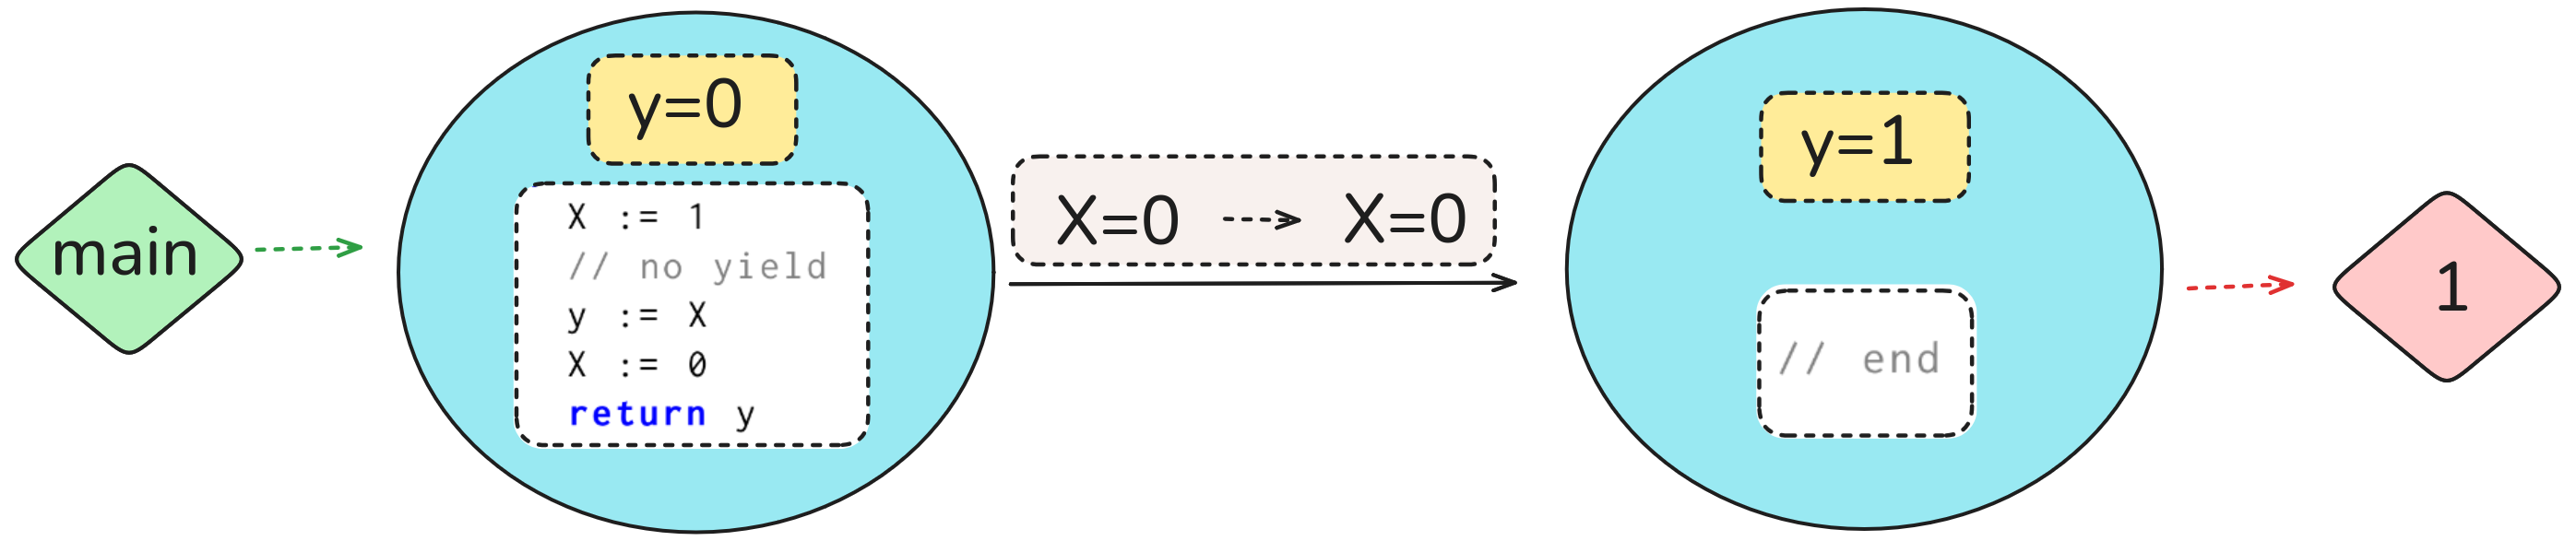
\includegraphics[width=0.9\textwidth]{plots/code_1_NS.png}
	\caption{Network System for interleaving executions of Listing~\ref{lst:MotivatingExample1Ser} program.}
	\label{fig:code1ExampleNS}
\end{figure}


\begin{figure}[htbp]
	\centering
	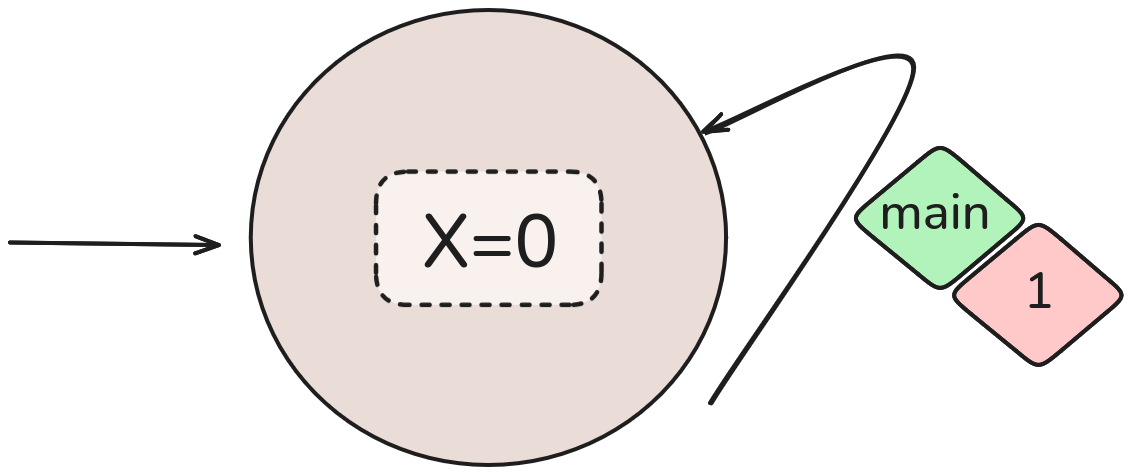
\includegraphics[width=0.4\textwidth]{plots/code_1_NFA.png}
	\caption{NFA for serialized executions of Listing~\ref{lst:MotivatingExample1Ser} program.}
	\label{fig:code1ExampleNFA}
\end{figure}



\begin{figure}[htbp]
	\centering
	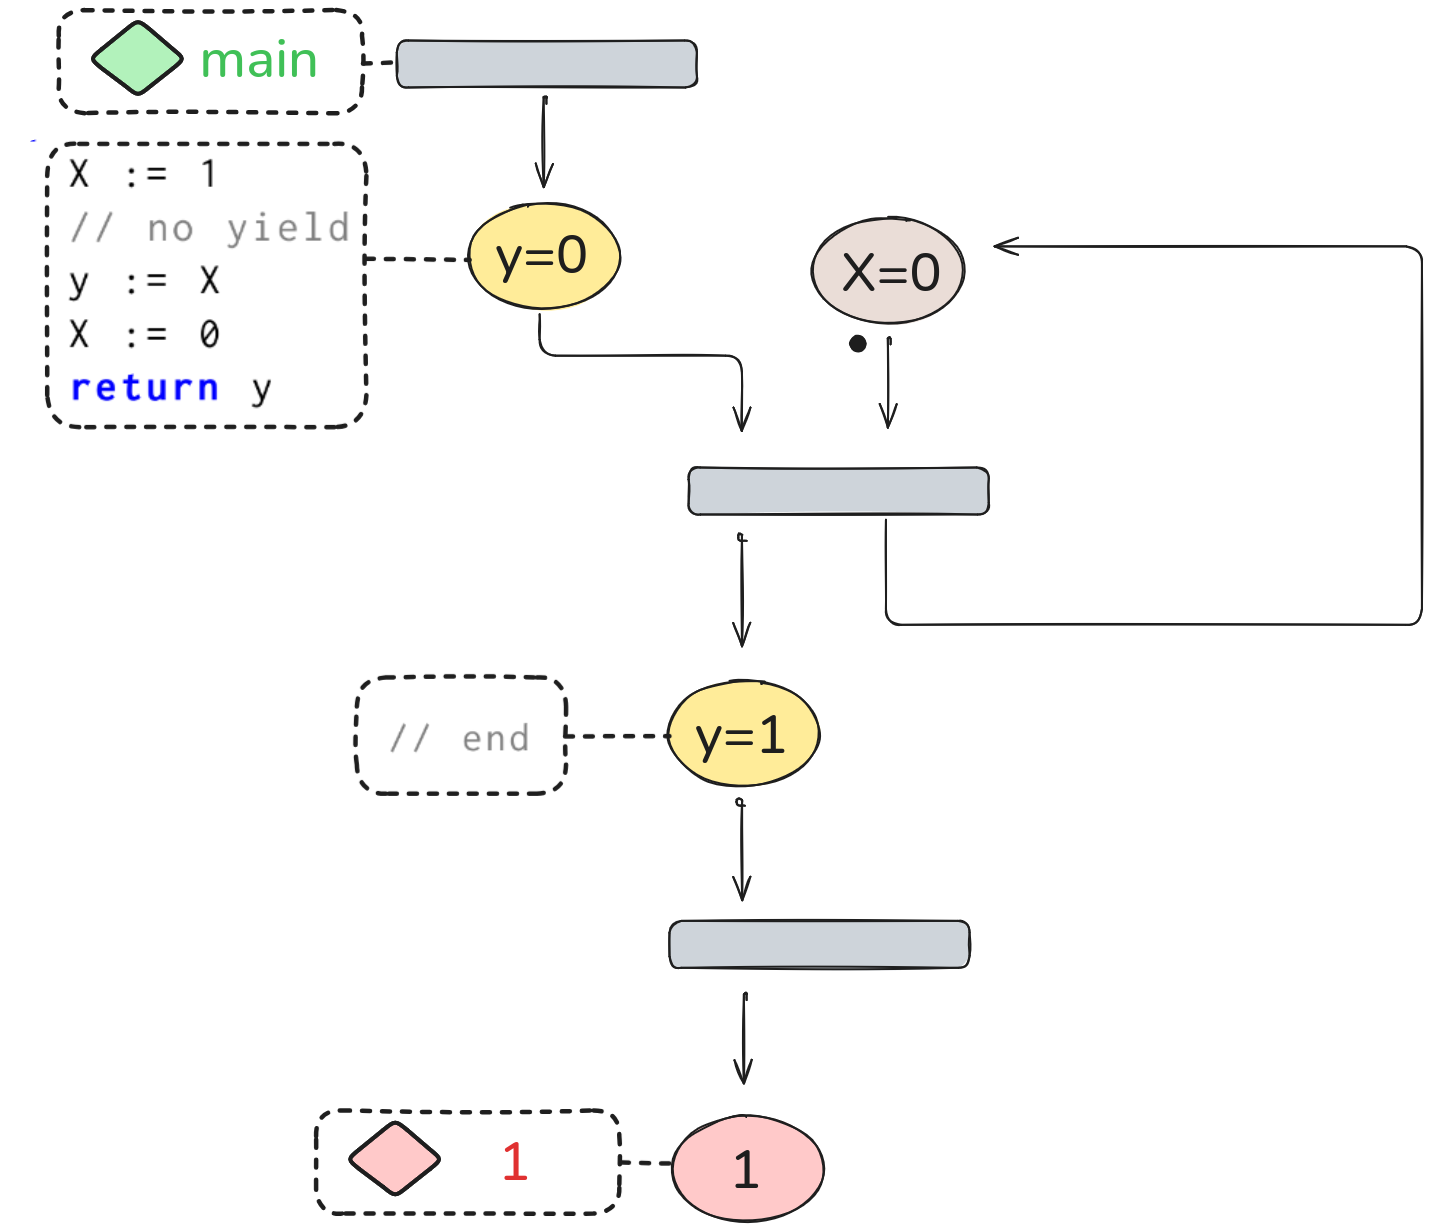
\includegraphics[width=0.5\textwidth]{plots/code_1_PN.png}
	\caption{Petri Net for interleaving executions of Listing~\ref{lst:MotivatingExample1Ser} program.}
	\label{fig:code1ExamplePN}
\end{figure}

%


\begin{figure}[htbp]
	\centering
	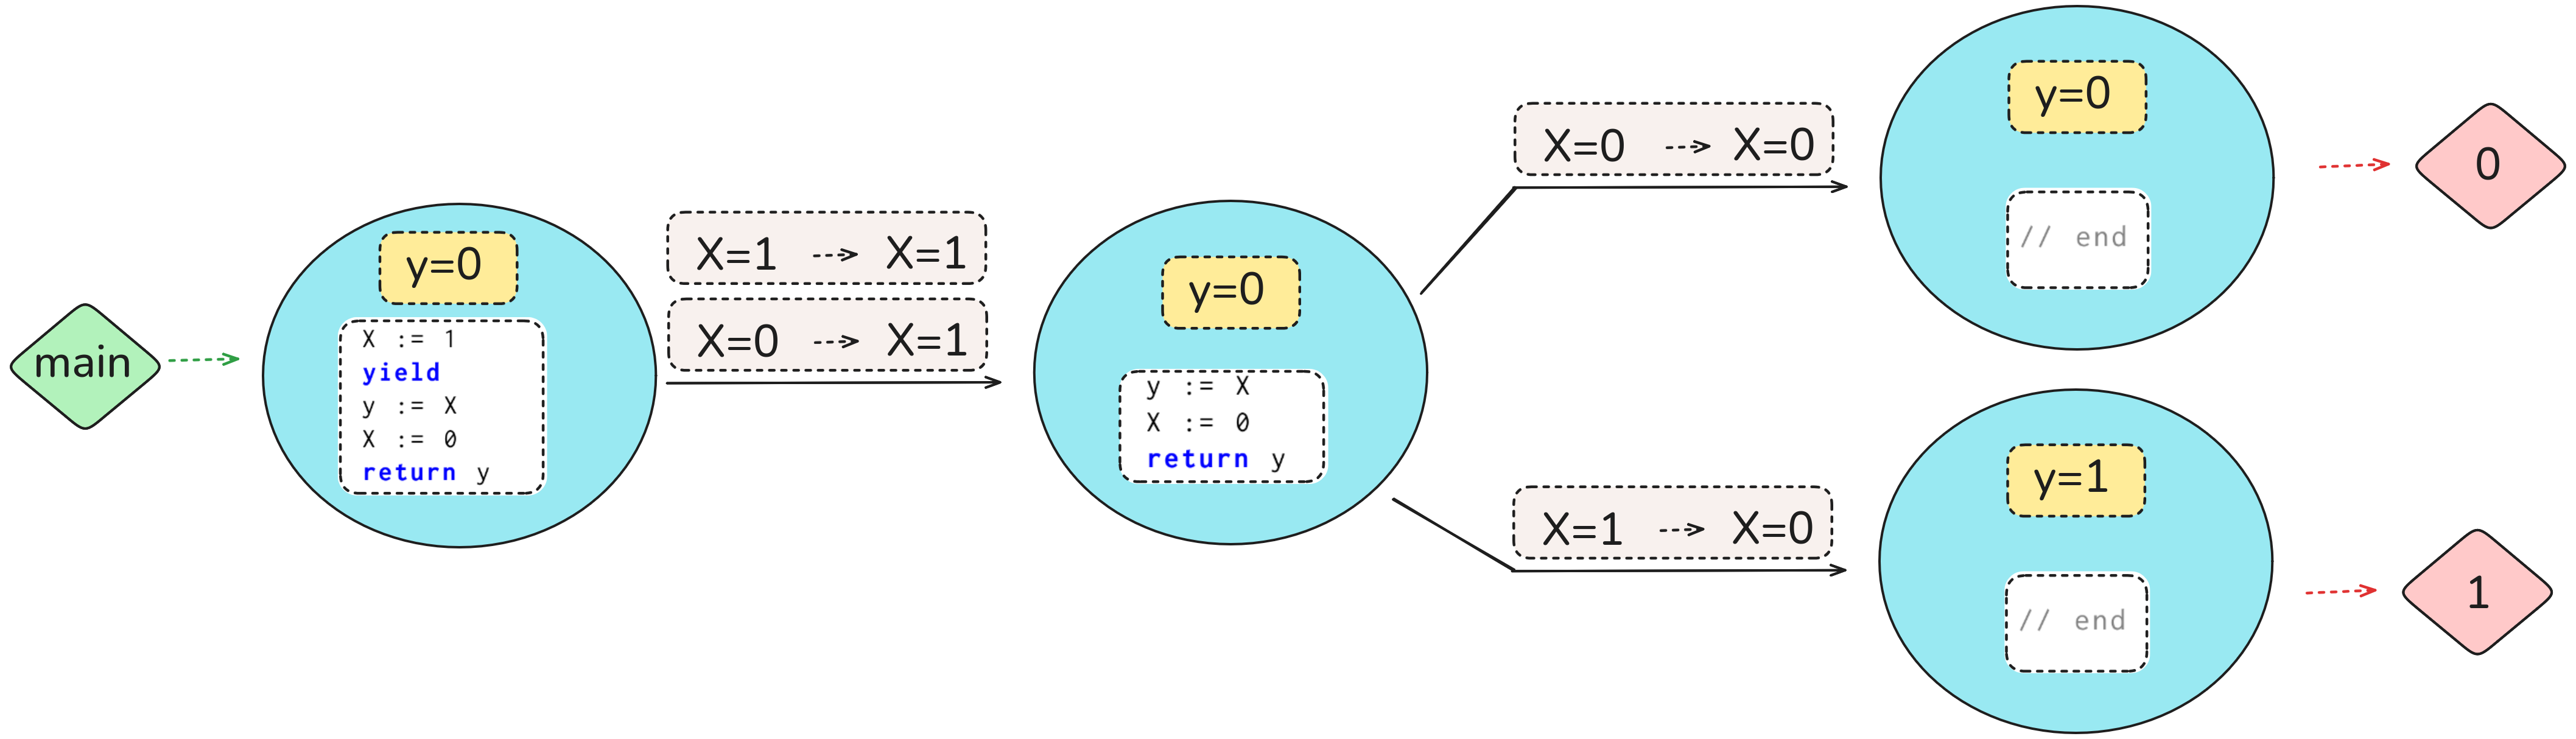
\includegraphics[width=1.1\textwidth]{plots/code_2_NS.png}
	\caption{Network System for interleaving executions of Listing~\ref{lst:MotivatingExample2NonSer} program.}
	\label{fig:code2ExampleNS}
\end{figure}


\begin{figure}[htbp]
	\centering
	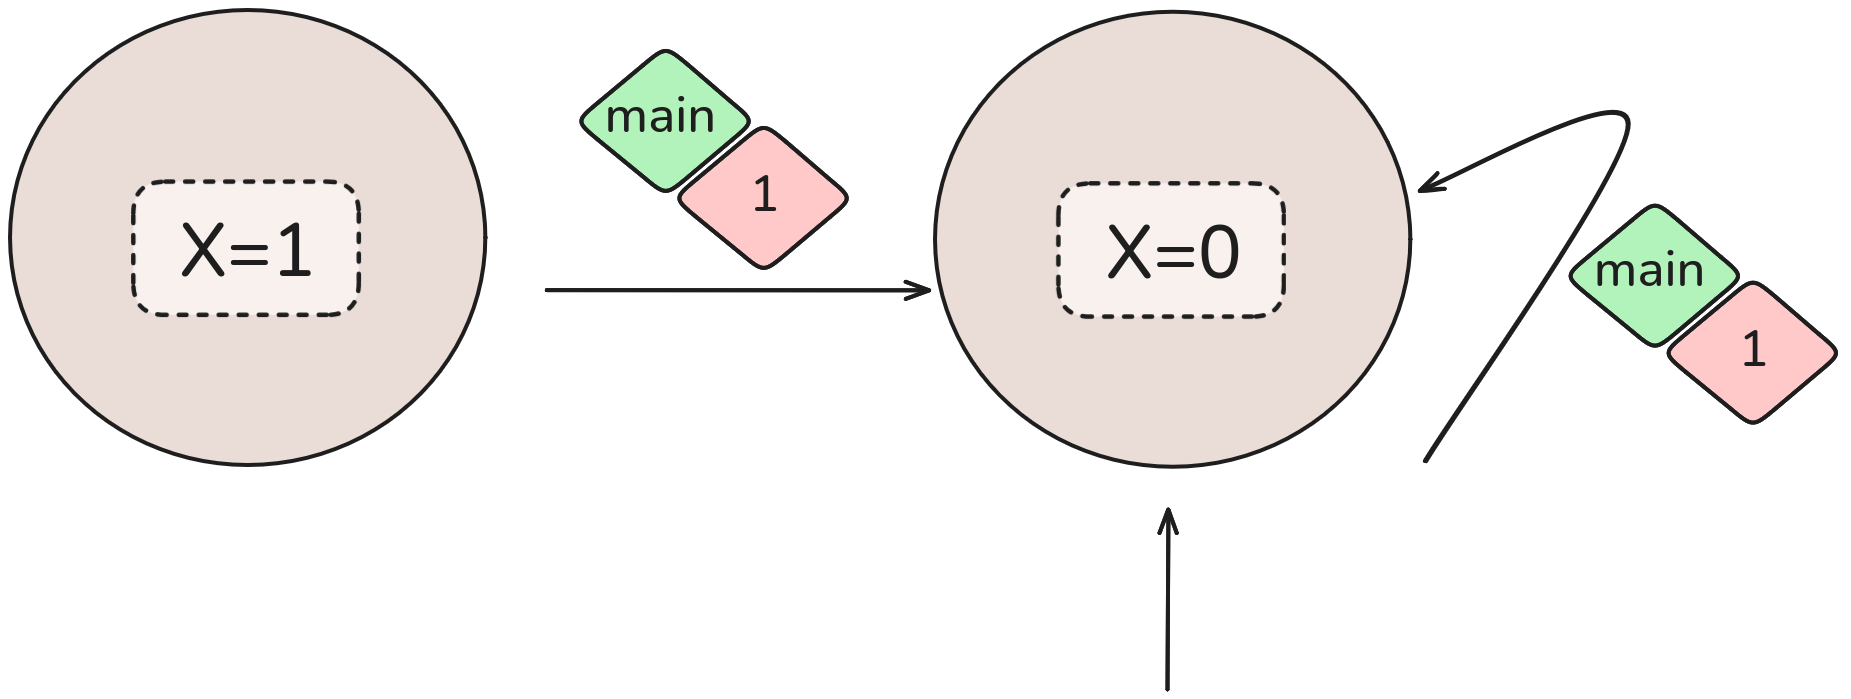
\includegraphics[width=0.6\textwidth]{plots/code_2_NFA.png}
	\caption{NFA for serialized executions of Listing~\ref{lst:MotivatingExample2NonSer} program.}
	\label{fig:code2ExampleNFA}
\end{figure}



\begin{figure}[htbp]
	\centering
	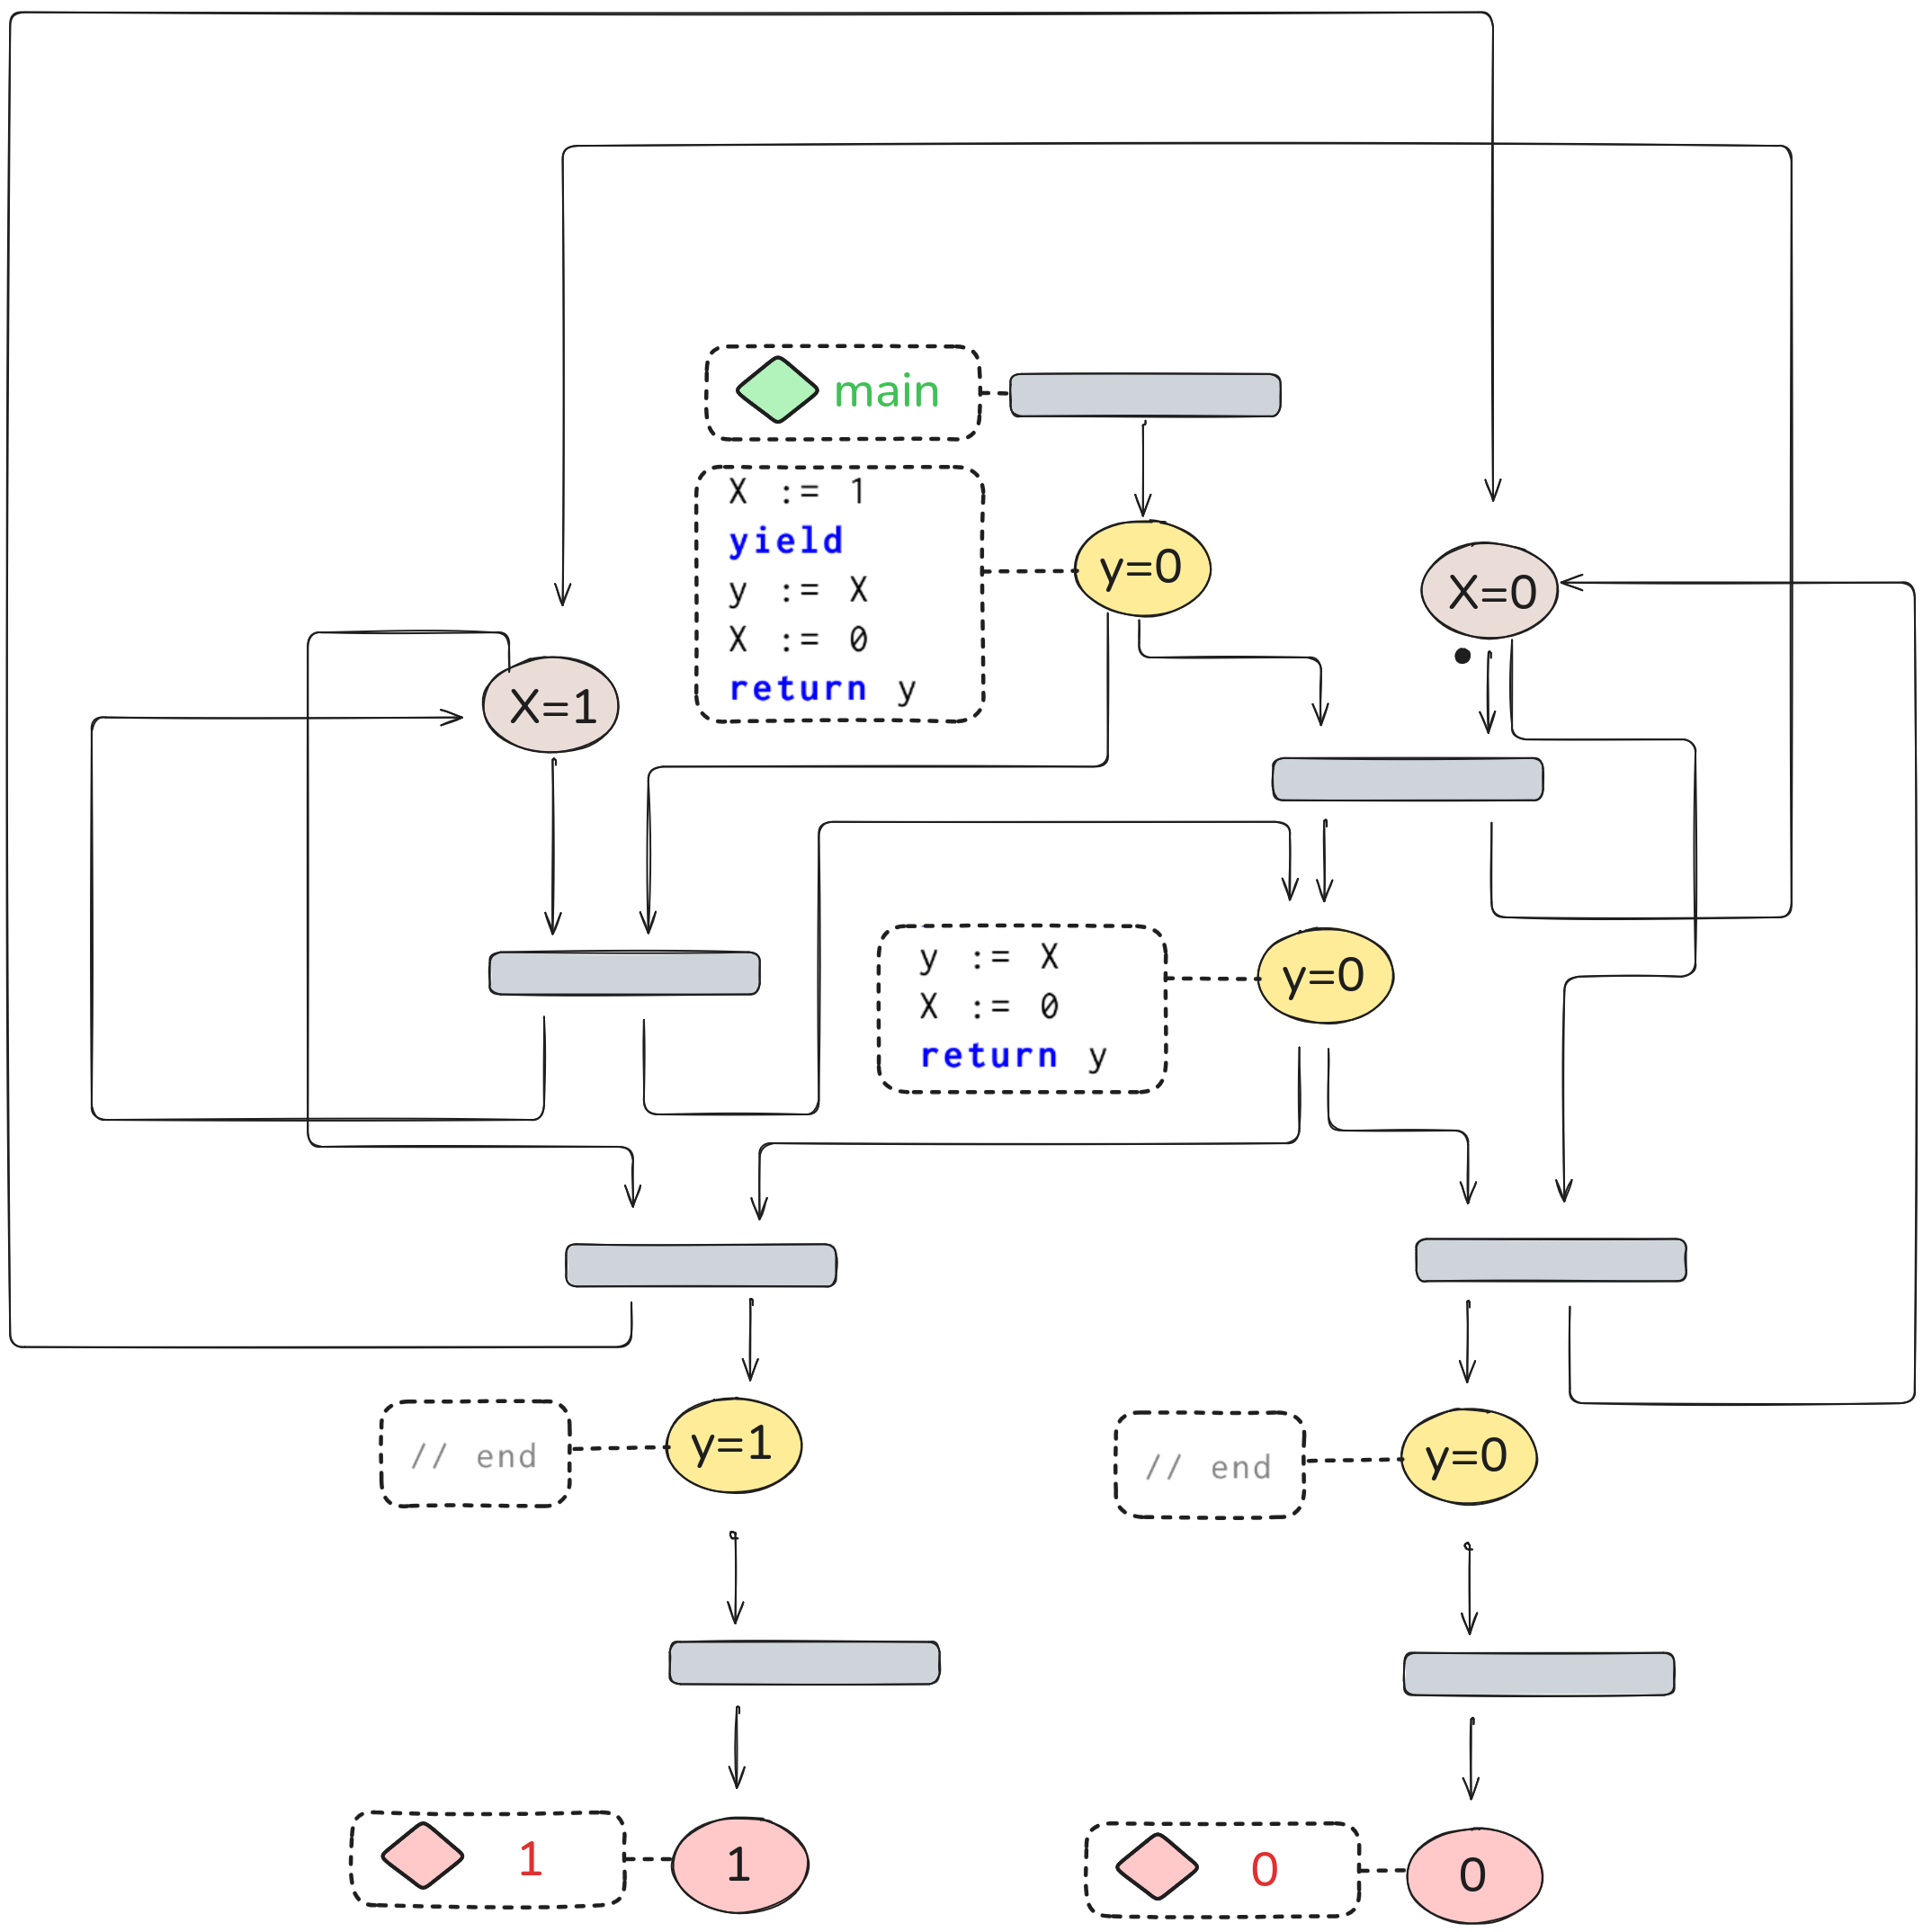
\includegraphics[width=0.7\textwidth]{plots/code_2_PN.png}
	\caption{Petri Net for interleaving executions of Listing~\ref{lst:MotivatingExample2NonSer} program.}
	\label{fig:code2ExamplePN}
\end{figure}



%


\begin{figure}[htbp]
	\centering
	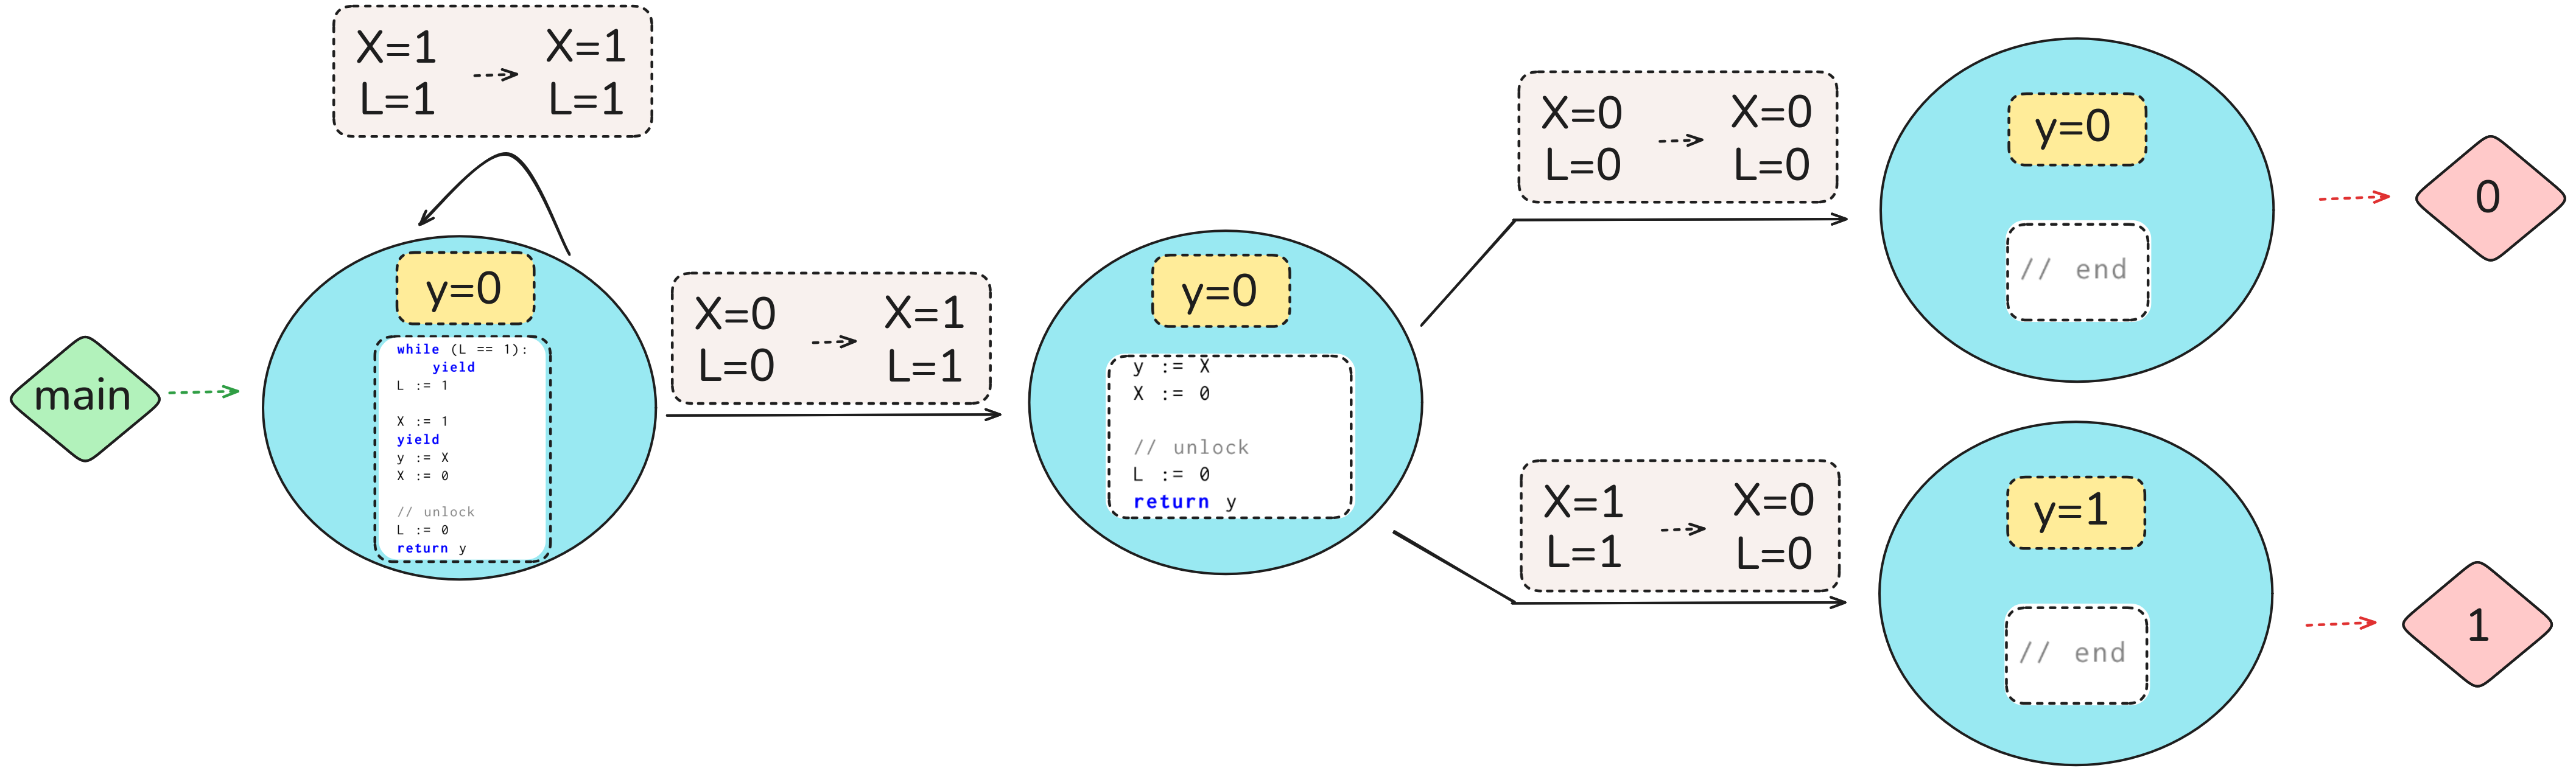
\includegraphics[width=1.1\textwidth]{plots/code_3_NS.png}
	\caption{Network System for interleaving executions of Listing~\ref{lst:MotivatingExample3Ser} program.}
	\label{fig:code3ExampleNS}
\end{figure}


\begin{figure}[htbp]
	\centering
	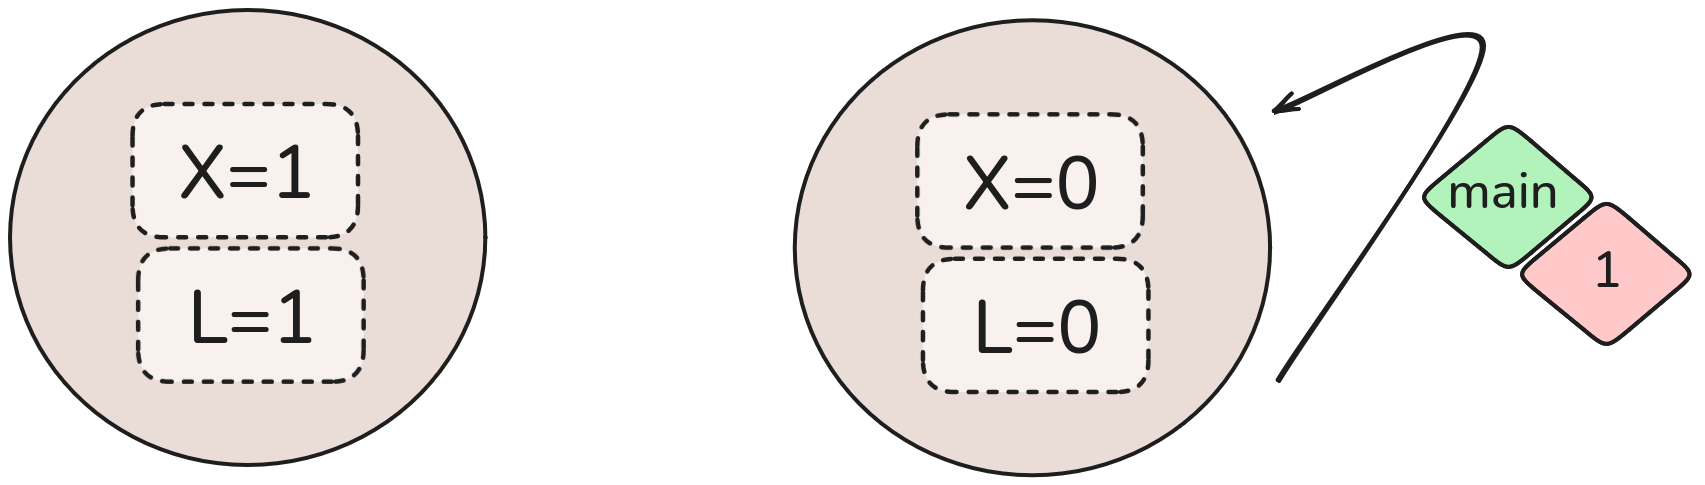
\includegraphics[width=0.6\textwidth]{plots/code_3_NFA.png}
	\caption{NFA for serialized executions of Listing~\ref{lst:MotivatingExample3Ser} program.}
	\label{fig:code3ExampleNFA}
\end{figure}



\begin{figure}[htbp]
	\centering
	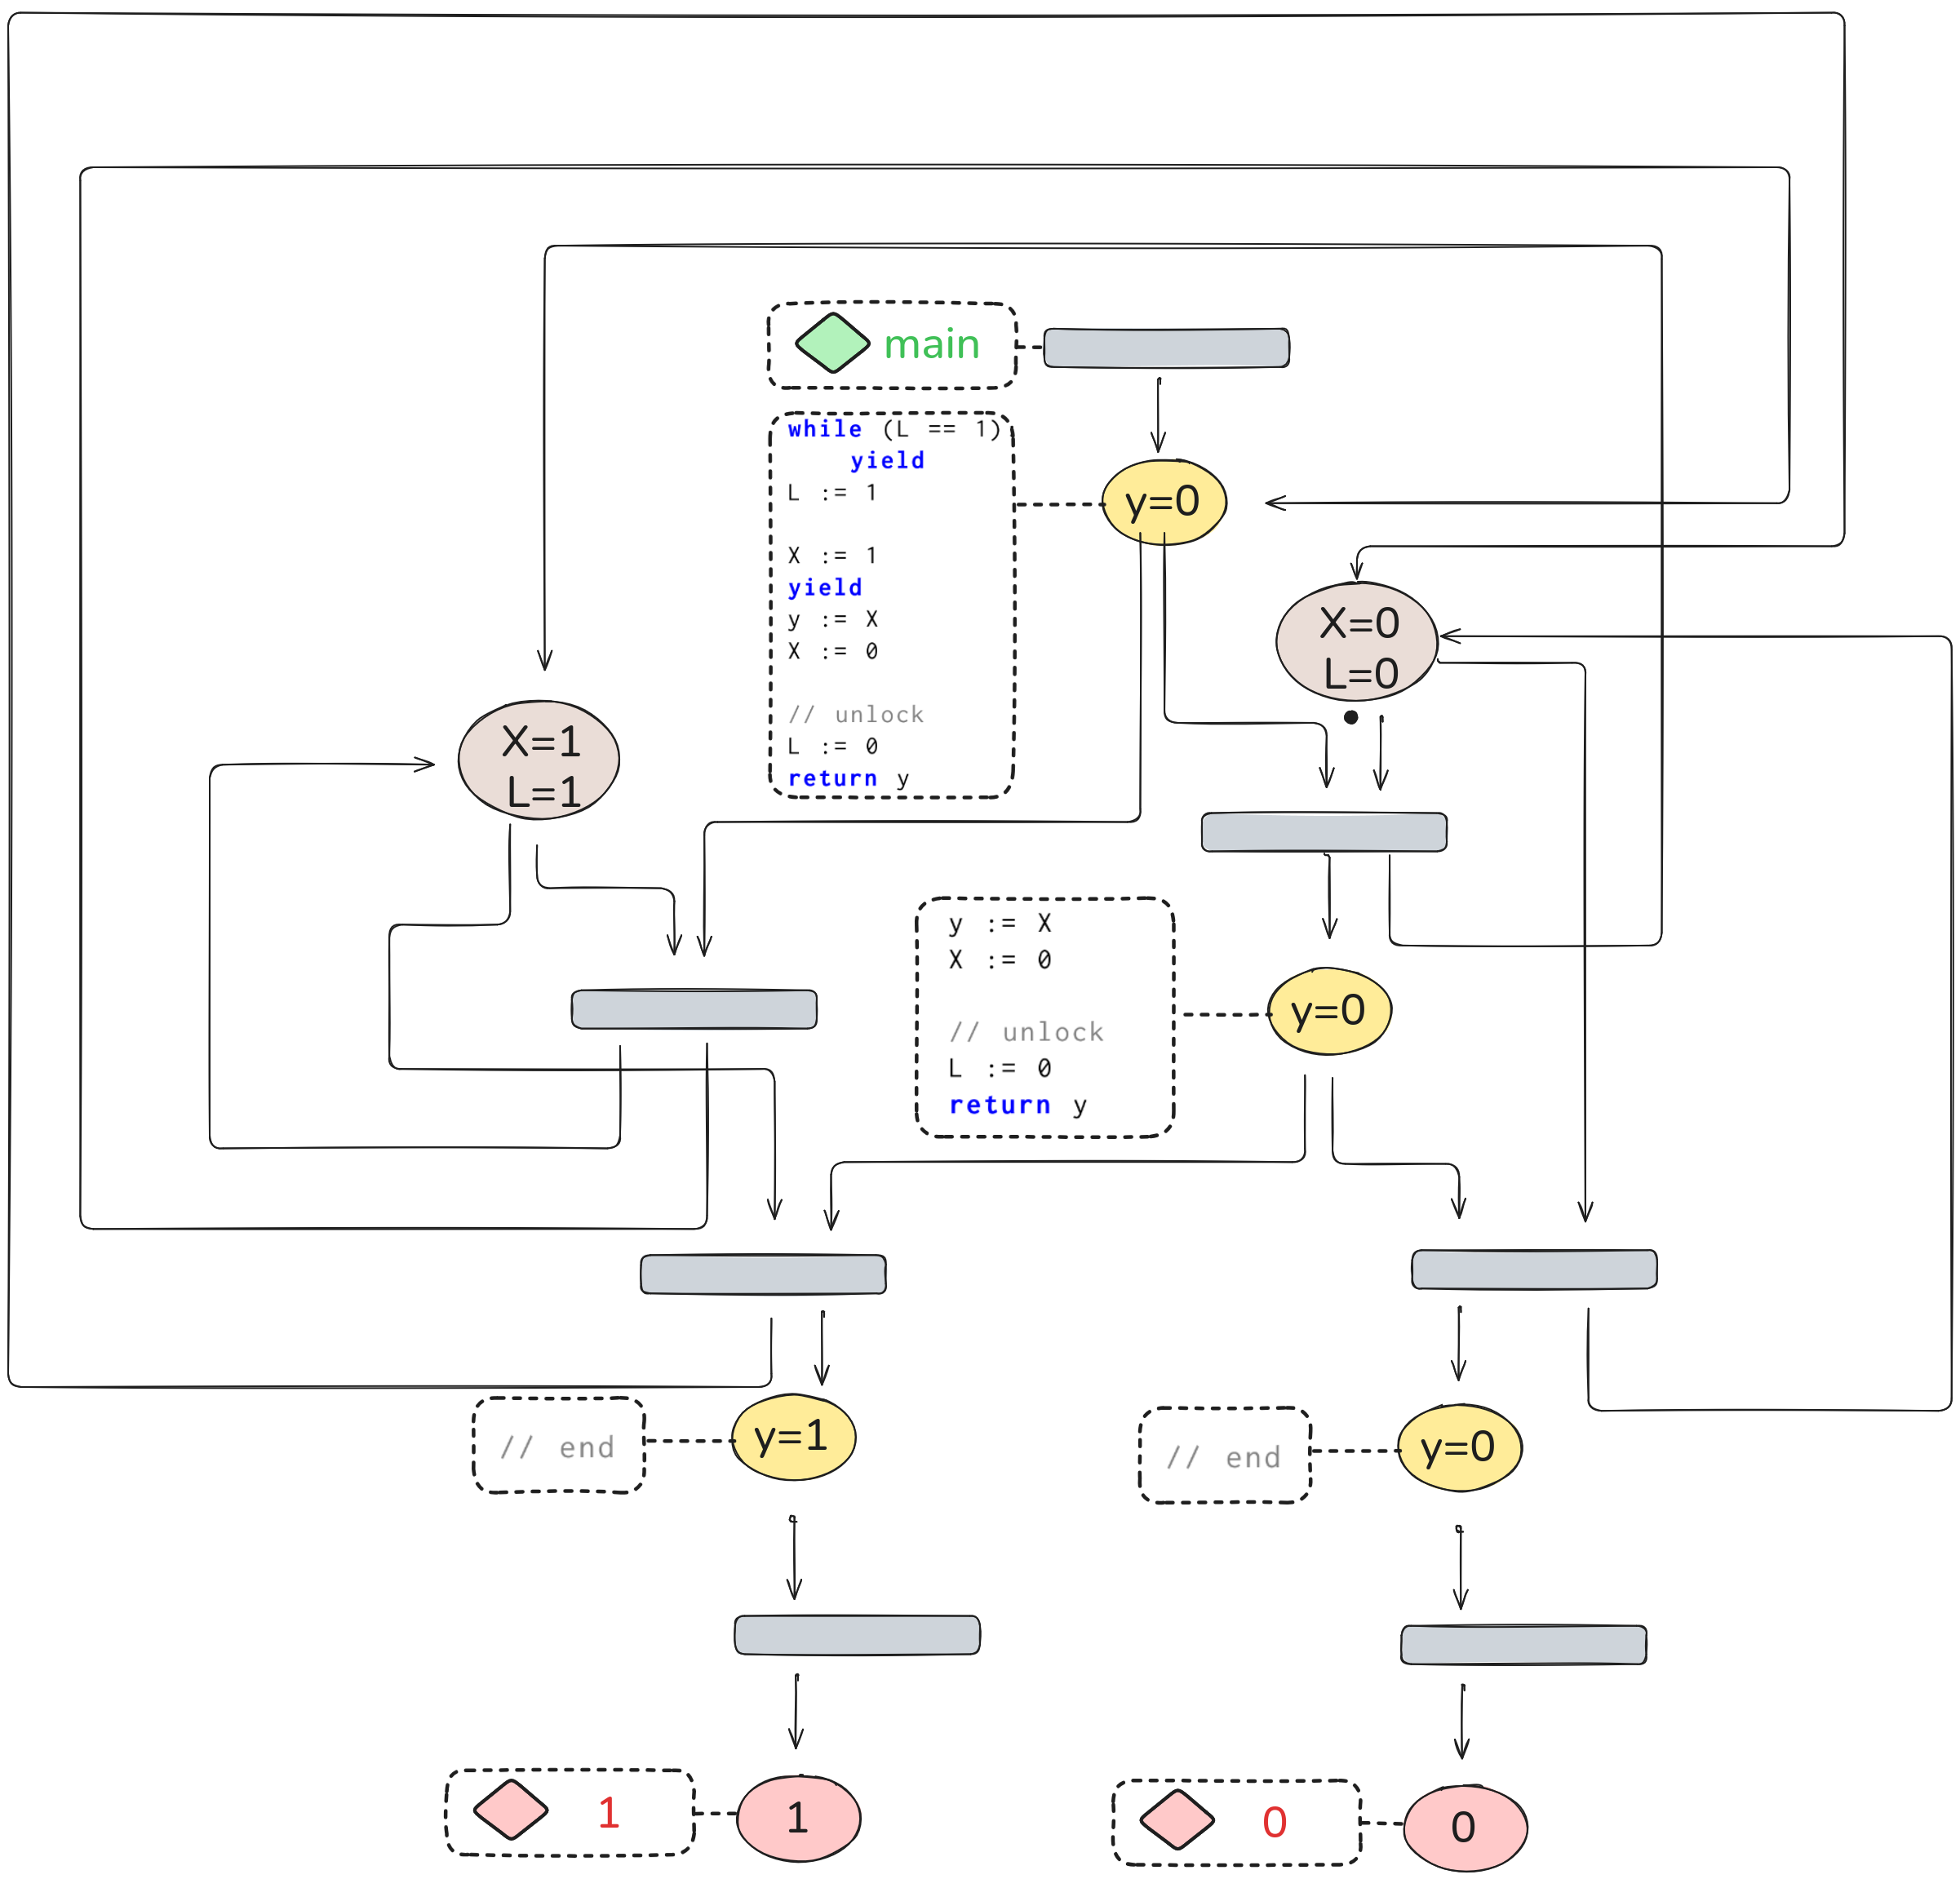
\includegraphics[width=0.8\textwidth]{plots/code_3_PN.png}
	\caption{Petri Net for interleaving executions of Listing~\ref{lst:MotivatingExample3Ser} program.}
	\label{fig:code3ExamplePN}
\end{figure}


\newpage